\documentclass[12pt]{article}
\usepackage{gensymb}
\usepackage{amsmath}
\usepackage{graphics}
\usepackage{graphicx}
\graphicspath{{storage/self/primary/Download/asgnt2/fig}}
\providecommand{\brak}[1]{\ensuremath{\left(#1\right)}}
\providecommand{\myvec}[1]{\ensuremath{\begin{pmatrix}#1\end{pmatrix}}}
\newcommand\norm[1]{\left\Vert#1\right\Vert}
\let\vec\mathbf
\begin{document}
\title{\textbf{ASSIGNMENT-12.11.2.3}}
\date{}
\maketitle
\textbf{Question :} Show that the line through the points \brak{4,7,8},\brak{2,3,4} is parallel to the line through the points\brak{-1,-2,1},\brak{1,2,5}.

\textbf{Solution :}
Line passing through \brak{4,7,8},\brak{2,3,4}is
\begin{align}
\frac{x-4}{1}=\frac{y-7}{2}=\frac{z-8}{2}\\
\end{align}
Direction vector,\begin{align}
    \vec{m_1}&=\myvec{1\\2\\2}
\end{align}
Line passing through \brak{-1,-2,1},\brak{1,2,5} is
\begin{align}
\frac{x+1}{1}=\frac{y+2}{2}=\frac{z-1}{2}
    \end{align}
Direction vector,\begin{align}
    \vec{m_2}&=\myvec{1\\2\\2}
\end{align}
Therefore,
\begin{align}
    \cos{\theta}&=\frac{\brak{\vec{m_1}}^{\top}\vec{m_2}}{\vec{\norm{m_1}\norm{m_2}}}\\
    &=\frac{\myvec{1&2&2}\myvec{1\\2\\2}}{9}\\
    &=1\\
    \implies \theta &= 0\degree
    \end{align}
\begin{figure}
    \centering
    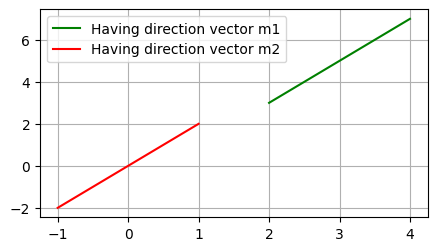
\includegraphics[width=\columnwidth]{fig/12.11.2.3.png}
    \caption{}
    \label{12.11.2.3}
\end{figure}
\end{document}

